\documentclass[letterpaper,fleqn]{article}

\usepackage[top=1in,bottom=1in,left=1in,right=1in]{geometry}
\usepackage{amsmath}
\usepackage{graphicx}
\usepackage{multirow}
\usepackage{float}
\usepackage{dirtree}
\usepackage{listings}
\usepackage{multicol}

\title{Project Hazzard\\ A Remotely Controlled Racing Adventure Game Experiment}
\author{Chen, Hao\\Nelson, Robert\\Stahl, Darren\\Vidanamadura, Hasith}

\begin{document}
\maketitle
\pagenumbering{gobble}
\pagebreak
\pagenumbering{arabic}

\section{Project Description}
Project Hazzard is a remote controlled racing game, using Raspberry Pis controlling one (or more) RC cars. Statistics about the cars current state (speed, direction, etc.) will be displayed on a GUI rendered using the Java \textsc{SWING} framework on a second Raspberry Pi. A third Raspberry Pi will be used to collect controller input from the players and forward that on to the Pis controlling the car's movements. Finally, a fourth Raspberry Pi will be attached through a GertBoard to the finish gate to detect when a car finishes a lap.

The separation of the controller from the controlled cars means that there can be additional influences added into the control path to add difficulty to the game. Any number of modifiers could be applied to challenge the players in their attempts to win the race.

\section{System Architecture}
\subsection{Deployment}
Project Hazzard is composed of 5 main subsystems. The input subsystem is responsible for processing input from Xbox controllers and passing the parsed values to the second subsystem PiNet. PiNet is responsible for allowing the other subsystems to communicate in a transparent manner. The game engine is responsible for processing all game logic and sending commands to the car subsystem. The car subsystem includes the scripts required to convert PiNet commands into car control signals, as well as the circuitry required to control the physical cars. The fourth subsystem is the finish gate. The finish gate detects when a car passes through it, and sends signals through PiNet to the game engine when it detects a car. The final subsystem, the GUI, is updated through PiNet by the game engine, and displays the current game state. Figure \ref{fig:deploy} shows the full deployment diagram. Each software subsystem is circled in a dashed line, and each hardware component is circled in a dot-dash line. All of the software components can be deployed to seperate Raspberry Pis if necessary, but they can also be deployed to the same Pi if that is more convenient.
\begin{figure}[ht]
\centering
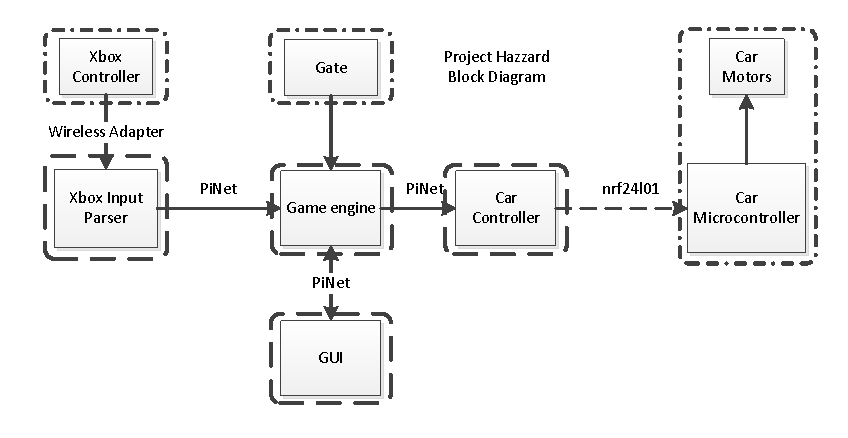
\includegraphics[width=0.75\textwidth]{Project-Block-Diagram-Deployment.pdf}
\caption{Deployment diagram for Project Hazzard}
\label{fig:deploy}
\end{figure}

\subsection{Communications}
Each of the four deployment components needs to communicate with each other. This communication is facilitated through PiNet, the networking library the team wrote for the trial project. Its flexibility allowed it to be easily ported into this application.

There are many different types of messages that are sent between the various components. Table \ref{tab:msgs} lists all of the various messages that each component sends and receives.
\begin{table}[H]
\centering
\caption{Messages sent and received by component}
\begin{tabular}{|l|r|r|} \hline
	Component & Messages Sent & Messages Received \\ \hline\hline
    Input Parser & ControllerEvent & XboxEvent \\ \hline
    \multirow{6}{*}{Game Engine} & RaceInfo & ControllerEvent \\
    & CarEvent & LapFinishedEvent \\
    & LapComplete & PingEvent \\
    & PlayerFinish & \\
    & RaceFinish & \\
    & PlayerInfo & \\ \hline
    Car Controller & & CarEvent \\ \hline
    Gate & LapFinishedEvent & \\ \hline
    \multirow{2}{*}{GUI} & & RaceInfo \\
    & & PlayerInfo \\ \hline
\end{tabular}
\label{tab:msgs}
\end{table}

\section{Class Diagrams}
Since each subsystem of the project was designed to be an independent module that performs in general, one function, a class diagram does not show much for most.
The class diagram for PiNet, which is used by most modules in the program serves to show how a class interacts with the PiNet classes. It is found in figure \ref{fig:pinet_uml}

\begin{figure}[H]
\centering
\includegraphics[width=\textwidth]{pinet_uml.PNG}
\caption{UML class diagram for PiNet, as used by any arbitrary class}
\label{fig:pinet_uml}
\end{figure}

\section{Sequence Diagrams}
A sequence diagram of the entire system would be far too large to be understandable, so smaller intercomponent sequence diagrams will be shown to detail the interaction between the components. Each sequence diagram will show one style of transaction that happens between the different components.

\subsection{Input}
The input subsystem encompases the Xbox controller, and the input controller. The sequence diagram for the behaviour of these systems can be seen in Figure \ref{fig:xbox_seq}

\begin{figure}[H]
\centering
\includegraphics{Xbox_Seq.png}
\caption{Sequence diagram for input subsystem}
\label{fig:xbox_seq}
\end{figure}

Input on the xbox controller is processed by the xpad driver, and converted into input events. These input events are read by the input library, and passed into the input controller. The input controller processes the events, performs rate limiting, and eliminates any unwanted events. Once only the desired events remain, the input events are converted into ControllerEvents and sent out over PiNet to the Game Engine.

\subsection{PiNet}
PiNet includes two methods of sending data to and from clients. The first is asyncronous data, the sequence diagram for which can be found in Figure \ref{fig:pinet_async}
Note: While both the following sequence diagrams show a single receiver, there can be any number of receivers.

\begin{figure}[H]
\centering
\includegraphics[width=0.75\textwidth]{pinet_async.PNG}
\caption{Sequence diagram for PiNet's async interface}
\label{fig:pinet_async}
\end{figure}

The other method PiNet provides is syncronous or update data. The sequence diagram for updates can be found in Figure \ref{fig:pinet_update}.

\begin{figure}[H]
\centering
\includegraphics[width=0.75\textwidth]{pinet_update.PNG}
\caption{Sequence diagram for PiNet's update interface}
\label{fig:pinet_update}
\end{figure}

\subsection{Game Engine}
The game engine has many different sequences that it procedes through, but for simplicity, only the most important one, the sequence that takes place during the race will be shown. The other sequences in the game engine are simply variations on Figure \ref{fig:game}, with some additional loops or checks.

\begin{figure}[H]
\centering
\includegraphics{Game_Engine_Seq.png}
\caption{Sequence diagram for the Game Engine during a race}
\label{fig:game}
\end{figure}

\subsection{RF Link}
The cars are connected to the main Raspberry Pi based network via a 2.4GHz-band radio network based on nRF24L01P modules. The modules provide auto-acknowledgement, and are reliable enough to perform at 1Mbps. The relevant documentation is given in the cuLearn book, and the sequence diagram (Figure \ref{fig:nrf}) showing the sequence of events when a radio packet is sent and processed by the car controller.

\begin{figure}[H]
\centering
\includegraphics{seq-nrf.png}
\caption{Sequence diagram for Raspberry Pi to Car Microcontroller communication}
\label{fig:nrf}
\end{figure}

\subsection{Car Microcontroller}
The cars are controlled by custom firmware running on AVR microcontrollers. These decode the RF link packets into commands to be forwarded to the actual car hardware. The microcontroller additionally supports the generation of the IR beacon for identifying cars. The sequence diagram in Figure \ref{fig:seq-car} identifies the decoding and beacon processes. For further information, please refer to the cuLearn book.

\begin{figure}[H]
\centering
\includegraphics[width=0.45\textwidth]{seq-cc.png}
\caption{Sequence diagram for Car Microcontroller activity}
\label{fig:seq-car}
\end{figure}
\section{Testing}
\subsection{Testing the Input Subsystem}
The input subsystem was difficult to test effectively due to its inherent dependency on the Xbox controller hardware. This made it impossible to write automated tests to check the input library code. Eventually, it was decided that since the code was relatively simple, a functional verification would be the only test. A test application was written to measure the rate that input events were received. Table \ref{tab:input_rate} shows the data collected during this test.

\begin{table}[H]
\centering
\caption{Number of input events observed during various input conditions}
\begin{tabular}{| l | c | c | c |} \hline
	\# of Controllers & No Input (Evts/s) & Normal Input (Evts/s) & Heavy Input (Evts/s) \\ \hline
    1 & 0 & ~120 & ~750 \\ \hline
    2 & 0 & ~250 & ~ 1600 \\ \hline
\end{tabular}
\label{tab:input_rate}
\end{table}

These test results led to the conclusion that the number of input events would exceed the capacity of PiNet if all of them were transmitted. The only recourse was to reduce the number of events by not sending any unnecessary events. The logical type of event to trim was the sensitivity of the analog values. Each analog stick had an X and Y range of -32767 to +32767. The cars only supported on/off turning, so these ranges were reduced to three values: -32767, 0, and +32767. All other analog events were ignored. This drastically reduced the number of events that needed to be sent to the game engine.

\subsection{Testing the RF link}
The major concern for the radios was reliability. Given that the modules themselves do not have external low-noise amplifiers or power amplifiers, the range of the modules was tested. To test this, the radios were plugged into the car microcontrollers, and disconnected from all outputs except serial for debugging. The idea was to monitor a continuous test (contained in ping\_test.c) that attempted to contact a target, and vary the distance and collect data.

\subsubsection{Effective Distance}

The \textbf{effective distance} is defined as the distance data can be transferred by a module transmitting at 0 $dBm$ (full power) with zero packets lost. The test application from the previous section was reused, and the module tested both in line of sight \textbf{(LOS)} and through-walls \textbf{(TW)} configurations.

Line of sight: The maximum testable line of sight distance was about 5m, and zero packet loss was observed.

Through-walls: The maximum distance testable was about 10m with two floors and walls between the source and the sink. Zero packet loss was observed even in that configuration. At 12m, noticeable packet loss (66\%) was observed.

Based on the above testing, the module meets the requirements. Since the project requires the cars to be visible to the players, the LOS configuration is more applicable, and the range in that configuration is sufficient for the purposes of this project. Further testing data including effects of the power rail noise is included in the cuLearn book.

\subsection{Testing PiNet}
PiNet was one of the few automated tests that could be done on the system, since each part relied so heavily on user input, or on physical output. 
PiNet/PiNetTest.py contains all of the testing code for PiNet. It starts by testing the small integral functions to make the system work, and slowly ramps the testing up to test more and more complicated parts. It eventually tests the system as a whole with fake inputs from a socket. It finishes by testing the system with the coresponding networking library partner.

\subsection{Testing the gate}
The gate is very reliant on its external surroundings, as it is based on light. Since it was built in an isolated location to get confirm its operation, even something as simple as running it in the lab was testing it. It was found that the flourescent lights triggered the sensor at 10KHz, which masked any cars driving though. It was required then that we block all light except for IR light. As a result of this test, an IR filter (magnetic disk from a floppy drive) was placed on the sensor, this prevented accidental trigger by the lights.

\section{Discussion}

\subsection{MVC}
The MVC model used in Project Hazzard is decentralized. It contains elements from multiple physical Raspberry Pis, as well as an abstract network packet. The controller is the Game Engine. The game engine is responsible for agregating the data from many sources, and compiling this data into a RaceInfo packet (the model), which is shared with the GUI (the view) over PiNet. This slightly deviates from the MVC model, in that a PiNet instance on the GUI does some networking and parsing of data, but it conforms to the spirit of MVC.

\subsection{XML}
XML is used in a number of places in the project. It is used to create a unified format for data in PiNet, and is used for configurations in the game engine.
\subsubsection{XML in PiNet}
In PiNet, XML is used to create a known format for sending the arguments to a callback, and a unified, extensible format for packaging classes. The callback uses a single element as the callback, and any number of attributes as the arguments. This is to limit the complexity of arguments, as they do not need to be extensible. The update data passing method uses all elements to store the data. This is because the class may contain multiple different types of data, which can be represented as a "type" attribute, or, may contain sub elements, which can be respresented as childen elements. This increased the load on the network, as there is a fairly large text overhead for using elements over attributes, but we felt that the ability to extend the update framework was worth the network overhead. A schema is not used, as the contents of the XML are unknown until execution time.
\subsubsection{XML for Powerups}
In the game engine, the powerups are stored as an XML configuration file (game\_engine/powerups.xml). This file follows a schema (game\_engine/powerups.xsd) which allows the game engine to ensure that each powerup follows the proper definition. GenerateDS, a tool which generates a python XML parser from an XML schema was used to create a class based parser for the powerups. Unfortunately, since the generated parser uses the SAX model to perform the parsing, the powerups file cannot be validated against the schema. Therefore, since the schema validation was an important step, a second XML library \textit{lxml} was used to ensure that the powerups were in a valid format.

The powerups format is very extensible, most data within a powerup is stored as elements. This provides the ability to add new elements in the future if for example more effects needed to be added. The name of the individual powerups however will always be required, and so that value is stored in an attribute on the top level \textit{powerup} element.

\section{Technical Recommendations}
While the individual components performed well in isolation, several issues cropped up during the presentation phase. After careful analysis, the following technical recommendations were agreed upon by the team.
\begin{enumerate}
\item The choice to use inexpensive RC cars as the hardware platform for the project was a mistake, as the cars required extensive retrofitting (to the level that none of the original electronics were retained), and performed less than expected. A revisiting of this project would replace the current RC cars with more dependable performance and reliability characteristics.


\item Time was wasted on attempting to port PiNet to Jython, so as to ease the interfacing with the 
(written in Java). Since Jython uses the underlying Java classes it was thought that this would be a simple way to interface the GUI with PiNet. 
Once the code had been converted to Jython, it was found that Jython did not support Multicasting, as the developers felt that it was not an important feature. This took a while to find out, and resulted in a large time sink when we needed it the least.
Once Jython was working by mixing Java and Python networking types, it still failed to integrate with the GUI. At this point, we had no choice but to cut our losses and rewrite PiNet in Java.

\item The order for the car controller PCB was placed in late October, as soon as the requirements for it were finalized. The delivery delays meant that the PCBs did not arrive until two weeks before the final presentation, unfortunately this caused a lot of the milestones to be missed, because they were scheduled based on the PCBs arriving when expected. The recommendation is therefore to overestimate how long it will take for PCBs to arrive, and plan accordingly. That way, if the boards arrive earlier than expected, there is extra time, but plans are in place if the boards are delayed.

\end{enumerate}
\section{README}
\subsection{Starting the System}
The system has several components, in order for the GUI to function properly
it must be started before the game engine. In addition, the RC cars must be started
before the car controller. All other components can be started in any order and the
system will function properly.

\subsubsection{Starting the GUI}

To start the GUI, the java files must be compiled using the commands:

\begin{lstlisting}
> cd GUI/src
> env CLASSPATH=com/hazzard/gui/dom4j-1.6.1.jar:com/hazzard/gui/jaxen-1.1.6.jar:.
	javac com/hazzard/gui/*.java
\end{lstlisting}

Then to run the GUI:

\begin{lstlisting}
> env CLASSPATH=com/hazzard/gui/dom4j-1.6.1.jar:com/hazzard/gui/jaxen-1.1.6.jar:.
	java com.hazzard.gui.Start
\end{lstlisting}

\subsubsection{Starting the Car Controller}

To run the car controller, the nrf library must be built.

Run:

\begin{lstlisting}
> make -C lib/bcm2835/
\end{lstlisting}

To build the library. Then, the car controller can be started by running:

\begin{lstlisting}
> cd car_controller
> ./car_controller.py
\end{lstlisting}

One thing to note is that the RC cars must be on before the car controller is started.

\subsubsection{Starting the Game Engine}

To run the game engine, simply run:

\begin{lstlisting}
> ./game_engine.py
\end{lstlisting}

\subsubsection{Starting the Input Controller}

To run the input controller, the xbox library must be built.

Run:

\begin{lstlisting}
> make -C xbox
\end{lstlisting}

and then the input controller can be started by executing

\begin{lstlisting}
> cd xbox
> ./input_controller.py
\end{lstlisting}

\subsubsection{Starting the Gate}
To run the gate, the shared library must be compiled

\begin{lstlisting}
> cd gate
> make
\end{lstlisting}

then, the Python wrapper must be started, it must be run as root to gain access to memory for GPIO actions; execute

\begin{lstlisting}
> sudo python wrapper.py
\end{lstlisting}

\subsection{Repository Layout}
\dirtree{%
  .1 /.
  .2 GUI.
  .3 build.
  .3 dist.
  .3 nbproject.
  .3 src.
  .2 PiNet.
  .3 examples.
  .2 car\_controller.
  .2 doc.
  .2 game\_engine.
  .2 gate.
  .2 lib.
  .3 avr.
  .3 bcm2835.
  .2 minutes.
  .2 weekly\_status.
  .2 xbox.
  }

\begin{itemize}
\item \textbf{GUI} contains the project for the Graphical User Interface.
\begin{itemize}
\item The source is located in \textbf{GUI/src/com/hazzard/gui}
\item The Netbeans project is located in \textbf{GUI/nbproject}.
\end{itemize}
\item PiNet sources are all located in \textbf{PiNet}.
\begin{itemize}
\item In \textbf{PiNet/examples} there are two examples, one of how to use a Sender and one of a Receiver.
\end{itemize}

\item \textbf{car\_controller} contains the Car Controller source.

\item \textbf{doc} contains the block diagrams of the system, and the presentations given.

\item \textbf{game\_engine} contains the central game engine and associated tests.

\item gate code is located in \textbf{gate}. It contains a make file, as well as sources.

\item \textbf{lib} is where the code for the car microcontroller, and the nrf24 radios is located.

\item \textbf{minutes} contains the meeting minutes for the meeting we have had.

\item weekly statuses are contained in \textbf{weekly\_status}, though there was only a few required.

\item \textbf{xbox} is where the code for parsing the xbox input resides.
\end{itemize}
\end{document}

